\documentclass[../main.tex]{subfiles}
\graphicspath{{\subfix{../Images/}}}

\begin{document}

\chapter{The Simplest Programs}

This chapter introduces Cg programming through a series of simple vertex and fragment programs. The chapter has the following four sections:

\FloatBarrier
\begin{itemize}
    \item \textbf{"A Simple Vertex Program"} presents a straightforward vertex program and explains the basic elements and syntax of the Cg language.
    \item \textbf{"Compiling Your Example"} explains how to compile programs for different GPUs, using the concept of profiles.
    \item \textbf{"A Simple Fragment Program"} defines a basic fragment program and introduces fragment profiles.
    \item \textbf{"Rendering with Your Vertex and Fragment Program Examples"} shows how to render simple geometry with OpenGL or Direct3D. This section also mentions the concept of clipping.
\end{itemize}
\FloatBarrier

\section{A Simple Vertex Program}

Green is the color associated with inexperience and growth, so a Cg program for rendering a green 2D triangle is a fitting way to start learning Cg.

Example 2-1 shows the complete source code for your first vertex program in Cg. Source code examples in this book use \textbf{boldface} to indicate Cg keywords, built-in functions, and built-in data types. This notation will help you identify words in programs that have special meaning to the Cg compiler. In addition, comments in code samples are set in gray type, to distinguish them from the rest of the code. Comments in Cg work just as in C++: you can use the \textbf{/*} and \textbf{*/} delimiters, or you can precede comments with the \textbf{//} characters.

\subsection*{The Naming Convention for Examples}

The vertex program in Example 2-1 is quite simple. The "\textbf{C2E1v}" prefix used in various parts of the program stands for "Chapter 2, Example 1 vertex program." We use this notation to make it easier to find examples across chapters and in the accompanying software framework. This convention makes it easier to keep track of the various examples in this book, but it is not a requirement of the Cg language itself and indeed is not a convention intended for your own programs.

\FloatBarrier
\begin{lstlisting}[caption=Example 2-1. The \textbf{C2E1v_green} Vertex Program]
struct C2E1v_Output {
  float4 position : POSITION;
  float4 color    : COLOR;
};

C2E1v_Output C2E1v_green(float2 position : POSITION)
{
  C2E1v_Output OUT;
  OUT.position = float4(position, 0, 1);
  OUT.color    = float4(0, 1, 0, 1);  // RGBA green
  return OUT;
}
\end{lstlisting}
\FloatBarrier

If you are familiar with C or C++, you can probably deduce what the program does. The program assigns the vertex's incoming 2D position to the vertex's output 2D position. In addition, it assigns the RGBA (red, green, blue, alpha) constant representing green to the output color of the vertex.

\subsection{Output Structures}

The \textbf{C2E1v_green} program begins with this declaration:

\FloatBarrier
\begin{lstlisting}
struct C2E1v_Output {
  float4 position : POSITION;
  float4 color : COLOR;
};
\end{lstlisting}
\FloatBarrier

This declaration is for a special structure known as an output structure. This structure contains the bundle of values that represent the output (or result) of a given Cg program.

A program written in a general-purpose CPU language such as C can perform a wide variety of tasks, such as reading and writing files, soliciting input from users, printing text, displaying graphics, and communicating over a network. Cg programs, on the other hand, are limited to outputting a bundle of values. A Cg program's output structure encapsulates the potential range of output values for a given Cg program.

Cg declares structures with the same syntax used in C and C++. A structure declaration begins with the struct keyword, followed by the name of the structure. Enclosed in curly brackets, a structure definition contains a list of structure members, each with a name and a type.

An output structure differs from a conventional C or C++ structure because it includes semantics for each member. We will return to the concept of semantics soon in Section 2.1.6.

\subsection{Identifiers}

When you declare a structure, you provide an identifier, or name, after the \textbf{struct} keyword; you do this for each structure you declare. An identifier in Cg has the same form as in C and C++. Identifiers consist of a sequence of one or more uppercase or lowercase alphabetic characters, the digits 0 to 9, and the underscore character (_). For example, \textbf{Matrix_B} and \textbf{pi2} are valid identifiers. An identifier cannot begin with a digit and cannot be a keyword.

Identifiers not only name structures, but also name type declarations, members of structures, variables, functions, and semantics (you will learn more about each of these shortly). Other identifiers in Example 2-1 are these:

\FloatBarrier
\begin{itemize}
\item \textbf{C2E1v_green} —the entry function name
\item \textbf{position} —a function parameter
\item \textbf{OUT} —a local variable
\item \textbf{float4} —a vector data type that is part of Cg's Standard Library
\item \textbf{color} and \textbf{position} —structure members
\item \textbf{POSITION} and \textbf{COLOR} —semantics
\end{itemize}
\FloatBarrier

Cg maintains different namespaces, based on the context of an identifier, in the same manner as C and C++. For example, the identifier \textbf{position} identifies a function parameter and a member of the \textbf{C2E1v_Output} structure.

\subsection*{Keywords in Cg}

Many Cg keywords are also C and C++ keywords, but Cg uses additional keywords not found in C or C++. Over the course of the book, we will explain most of these keywords. Appendix D contains the complete list of Cg keywords. As in C and C++, Cg's keywords are not available for use as identifiers.

\subsection{Structure Members}

Within the curly brackets of a structure declaration, you will find one or more structure members. Each member is a data type with an associated member name.

In the \textbf{C2E1v_Output} structure, there are two members: \textbf{position} and \textbf{color}. Both members are four-component floating-point vectors, as indicated by their type, \textbf{float4}.

\subsection{Vectors}

The fundamental data types in C or C++ are scalar quantities, such as \textbf{int} or \textbf{float}. In C or C++, there is no native "vector" type, so vectors are typically just arrays of scalar values. Because vectors are essential to vertex and fragment processing and because GPUs have built-in support for vector data types, Cg has vector data types.

The members (\textbf{position} and \textbf{color}) are declared using the \textbf{float4} data type. This name is not a reserved word in Cg; it is a standard type definition in the Cg Standard Library. Unlike in C and C++, there is no need to specify a preprocessor statement (such as \textbf{\#include}) to include declarations for Cg's Standard Library. Instead, Cg automatically includes the declarations needed by most Cg programs.

You should rely on the predefined vector data types provided by the Cg Standard Library, such as \textbf{float2}, \textbf{float3}, \textbf{float4}, and other such types to ensure that your programs make the most efficient use of the vector processing capabilities of your programmable GPU.

\subsection*{Advanced}

Vector types in Cg, such as \textbf{float3} and \textbf{float4}, are not 100 percent equivalent to arrays of however many \textbf{float}s. For example, \textbf{float x[4]} is not the same declaration as \textbf{float4 x}. These vector types are, in fact, \textit{packed arrays}. Packed arrays, often just called vectors, tell the compiler to allocate the elements of packed arrays so that vector operations on these variables are most efficient. If two input vectors are stored in packed form, programmable graphics hardware typically performs three-component or four-component math operations—such as multiplications, additions, and dot products—in a single instruction.

Packed arrays are not available in conventional programming languages like C and C++. Recent CPU instruction sets—such as Intel's SSE2, SSE, and MMX; AMD's 3DNow!; and Motorola's AltiVec—have additional vector instructions, but packed arrays are not natively supported by most general-purpose programming languages. Cg, however, provides specific support for packed arrays because vector quantities are integral to vertex and fragment processing. Packed arrays help the Cg compiler take advantage of the fast vector operations provided by programmable GPUs.

As with many aspects of Cg, how you use packed arrays depends on the Cg profile you select. For example, packed arrays are usually limited to four or fewer components. They are often extremely efficient for vector operations such as assignment, negation, absolute value, multiplication, addition, linear interpolation, maximum, and minimum. Dot-product and cross-product operations with packed operands are also very efficient.

On the other hand, accessing packed arrays with a nonconstant array index is either inefficient or unsupported, depending on the profile. For example:

\FloatBarrier
\begin{lstlisting}
float4 data = { 0.5, -2, 3, 3.14159 }; // Initializer,
                                       // as in C
int index = 3;
float scalar;
scalar = data[3];     // Efficient
scalar = data[index]; // Inefficient or unsupported
\end{lstlisting}
\FloatBarrier

The rule of thumb is to declare all vectors that consist of two, three, or four components (such as colors, positions, texture coordinate sets, and directions) as packed arrays by using Cg's built-in vector types.
\hrule

\subsection{Matrices}

In addition to vector types, Cg natively supports matrix types. Here are some examples of matrix declarations in Cg:

\FloatBarrier
\begin{lstlisting}
float4x4 matrix1; // Four-by-four matrix with 16 elements
half3x2 matrix2;  // Three-by-two matrix with 6 elements
fixed2x4 matrix3; // Two-by-four matrix with 8 elements
\end{lstlisting}
\FloatBarrier

You can declare and initialize a matrix with the same notation that would be used to initialize an array in C or C++:

\FloatBarrier
\begin{lstlisting}
float2x3 matrix4 = { 1.0, 2.0,
                     3.0, 4.0,
                     5.0, 6.0 };
\end{lstlisting}
\FloatBarrier

Like vectors, matrices are packed data types in Cg, so operations using standard matrix types execute very efficiently on the GPU.

\subsection{Semantics}

A colon and a special word, known as a semantic, follow the \textbf{position} and \textbf{color} members of the \textbf{C2E1v_Output} structure. Semantics are, in a sense, the glue that binds a Cg program to the rest of the graphics pipeline. The semantics \textbf{POSITION} and \textbf{COLOR} indicate the hardware resource that the respective member feeds when the Cg program returns its output structure. They indicate how the variables preceding them connect to the rest of the graphics pipeline.

The \textbf{POSITION} semantic (in this case, in an output structure used by a Cg vertex program) is the clip-space position for the transformed vertex. Later graphics pipeline stages will use the output vector associated with this semantic as the post-transform, clip-space position of the vertex for primitive assembly, clipping, and rasterization. You will be introduced to clip space later in this chapter, and more formally in Chapter 4. For now, you can think of a 2D vertex's clip-space position simply as its position within a window.

The \textbf{COLOR} semantic in this context is what Direct3D calls the "diffuse vertex color" and OpenGL calls the "primary vertex color." Color interpolation for a triangle or other geometric primitive during rasterization depends on the primitive's per-vertex colors.

\subsection*{Caution}

Do not confuse a member name with its semantic. In Example 2-1, the \textbf{position} member is associated with the \textbf{POSITION} semantic. However, it is the use of the \textbf{POSITION} semantic after the member name—not the name of the member itself—that makes the rasterizer treat the \textbf{position} member as a position. In the following output structure, the member names \textbf{density} and \textbf{position} are poorly chosen, but Cg abides by the specified semantics despite the misleading names:

\FloatBarrier
\begin{lstlisting}
struct misleadingButLegal {
  float4 density  : POSITION; // Works, but confusing
  float4 position : COLOR;   // Also confusing
};
\end{lstlisting}
\FloatBarrier
\hrule

Subsequent examples will introduce other output semantic names. Not all semantics are available in all profiles, but in our examples, we will use the semantics that are broadly supported by existing profiles.

You can also create your own semantic names, but in this book, we limit our examples to the standard set of semantics. For more information about using your own semantic names, see the \textit{Cg Toolkit User's Manual: A Developer's Guide to Programmable Graphics}.

\subsection{Functions}

Declaring functions in Cg works in much the same way as it does in C and C++. You specify a return type for the function (or \textbf{void} if nothing is returned), its name, and a comma-separated parameter list in parentheses. After the declaration, the body of the function describes the computation performed by the function.

Functions can be either entry functions or internal functions.

\subsection*{Entry Functions}

An \textit{entry function} defines a vertex program or fragment program; it is analogous to the \textbf{main} function in C or C++. A program's execution starts in its entry function. In Example 2-1, the entry function called \textbf{C2E1v_green} is defined as follows:

\FloatBarrier
\begin{lstlisting}
C2E1v_Output C2E1v_green(float2 position : POSITION)
\end{lstlisting}
\FloatBarrier

This function returns the output structure \textbf{C2E1v_Output} described earlier. This means that the function outputs both a position and a color. These outputs have semantics defined by the structure.

The function also accepts an input parameter named \textbf{position} . This parameter has the type \textbf{float2}, so it is a floating-point vector with two components. When a colon and semantic name follow an input parameter name, this indicates the semantic associated with that input parameter. When \textbf{POSITION} is used as an input semantic, this tells the vertex processor to initialize this parameter with the application-specified position of every vertex processed by the function.

\subsection*{Internal Functions}

\textit{Internal functions} are helper functions called by entry functions or other internal functions. You can use the internal functions provided by the Cg Standard Library, and you can define your own internal functions as well.

Internal functions ignore any semantics applied to their input or output parameters or return values; only entry functions use semantics.

\subsection{Input and Output Semantics Are Different}

Figure \ref{fig:2-1} shows the flow of input and output semantics for the \textbf{C2E1v_green} vertex program.

\begin{figure}
    \centering
    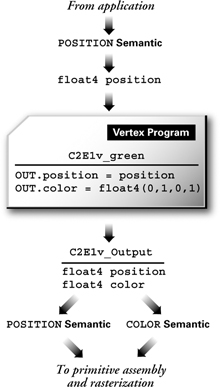
\includegraphics[width=0.5\linewidth]{fig2_1.jpg}
    \caption{The Flow of Semantic Inputs and Outputs for \textbf{C2E1v_green}}
    \label{fig:2-1}
\end{figure}

Input and output semantics are not the same, even though some have the same names. For example, for an input parameter to a vertex program, \textbf{POSITION} refers to the application-specified position assigned by the application when it sends a vertex to the GPU. However, an output structure element with the \textbf{POSITION} semantic represents the clip-space position that is fed to the hardware rasterizer.

Both semantics are named \textbf{POSITION} and, indeed, each is a position. However, each position semantic refers to a position at different points along the graphics pipeline. Your Cg vertex program transforms the application-supplied vertex position into a vertex suited for primitive assembly, clipping, and rasterization. In the \textbf{C2E1v_green} program, this transformation is trivial (the vertex position is passed along unchanged), but later in this book, particularly in Chapters 4 and 5, you will learn more useful and interesting ways to transform vertices.

\subsection{The Function Body}

The substance of the \textbf{C2E1v_green} function is contained in its body:

\FloatBarrier
\begin{lstlisting}
{
  C2E1v_Output OUT;
  OUT.position = float4(position, 0, 1);
  OUT.color    = float4(0, 1, 0, 1);  // RGBA green
  return OUT;
}
\end{lstlisting}
\FloatBarrier

Because the function's return type is \textbf{C2E1v_Output}, you must declare a variable of this type to hold the value that the function returns. We often call a structure returned by an entry function an \textit{output structure}. The function body sets both elements of this structure variable and returns the structure. (Note that the entry function's return type is not required to have the same prefix as the entry function, although we've chosen to make them the same in our examples.)

The dot between \textbf{OUT} and \textbf{position}, as well as \textbf{OUT} and \textbf{color}, is the \textit{member operator} and gives access to a member within a structure. This is the same way that C and C++ access structure members. Think of a structure as a container for multiple values. The member operator lets you retrieve the values contained in a structure:

\FloatBarrier
\begin{lstlisting}
   OUT.position = float4(position, 0, 1);
   OUT.color    = float4(0, 1, 0, 1); // RGBA green
\end{lstlisting}
\FloatBarrier

First, the program assigns the \textbf{position} input parameter to \textbf{OUT.position}. However, the output structure member \textbf{OUT.position} is of type \textbf{float4} (Chapter 4 explains why). The expression \textbf{float4 (position, 0, 1)} converts a two-component position vector to a four-component vector by setting the third and fourth components to 0 and 1, respectively.

Second, the program assigns the RGBA color value for green to \textbf{OUT.color}. To provide the numeric value for green, construct the appropriate four-component color vector. The type of the \textbf{color} member is \textbf{float4} because the color is an RGBA color. The "A" in RGBA stands for "alpha," which normally encodes a measure of how opaque or transparent a color value is. The value 1 for alpha means the color is fully opaque.

When you use the \textbf{float4} or similar vector type name like a function (for example, \textbf{float4(0, 1, 0, 1)}), this is a called a \textit{constructor}. This constructor creates a value of the type specified out of the values listed in the parentheses. C++ has the concept of constructors, but C does not. Constructors in Cg are provided for vectors and matrices.

The syntax \textbf{float4(0, 1, 0, 1)} creates a vector <0, 1, 0, 1> that is assigned to the \textbf{color} member of type \textbf{float4} in \textbf{OUT}. The vector <0, 1, 0, 1> is green because the color components are in the red, green, blue, alpha (RGBA) order with a green (and alpha) contribution specified, but no red or blue contribution.

\FloatBarrier
\begin{lstlisting}
    return OUT;
\end{lstlisting}
\FloatBarrier

Finally, the \textbf{return} statement returns the output structure you initialized. The collection of values within \textbf{OUT} is passed along to the next stage of the graphics pipeline, as indicated by the semantics assigned to each member.

\section{Compiling Your Example}

You use the Cg runtime to load and compile Cg programs. When you compile a program, you must specify two things in addition to the text of the program:

\FloatBarrier
\begin{itemize}
\item The name of the entry function to compile
\item The profile name for the entry function to compile
\end{itemize}
\FloatBarrier

The name of the entry function in Example 2-1 is \textbf{C2E1v_green} .

\textbf{C2E1v_green} is a vertex program, so you need to compile for a vertex profile. The vertex profile you choose depends on the programming interface your application uses for 3D rendering (OpenGL or Direct3D), as well as the hardware capabilities of your GPU.

\subsection{Vertex Program Profiles}

There are several appropriate vertex profiles for compiling our example, as listed in Table \ref{table:2-1}. Future GPUs will no doubt support profiles that are more capable.

\begin{table}
\centering
\begin{tabular}{ |c|c|c|c|c|c|c|c| } 
 \hline
Profile Name & Programming Interface & Description \\
arbvp1 & OpenGL & Basic multivendor vertex programmability (corresponding to ARB_vertex_program functionality) \\
vs_1_1 & DirectX 8 & Basic multivendor vertex programmability \\
vp20 & OpenGL & Basic NVIDIA vertex programmability (corresponding to NV_vertex_program functionality) \\
vs_2_0 vs_2_x & DirectX 9 & Advanced multivendor vertex programmability \\
vp30 & OpenGL & Advanced NVIDIA vertex programmability (corresponding to NV_vertex_program2 functionality) \\
 \hline
\end{tabular}
\caption{Cg Vertex Profiles}
\label{table:2-1}
\end{table}

Your first example is very simple, so there is no problem compiling it with any of the profiles in Table 2-1, or any future vertex profile for that matter. As you progress through the book, you'll encounter some complex Cg programs that will require advanced vertex or fragment profiles. When an advanced profile is required, we are careful to point that out. Most examples in this book are written to compile for a broad range of Cg profiles.

Because you'll want your \textbf{C2E1v_green} example to compile on the broadest range of GPUs, the best profiles for your example are \textbf{arbvp1} for OpenGL and \textbf{vs_1_1} for DirectX 8. Is there any reason to choose another profile? Yes, if you want to use advanced vertex programmability functionality, such as complex flow control or fast hardware instructions, which are not available in the basic profiles. For example, if you choose the \textbf{vp30} profile, you can write a Cg vertex program that loops a varying (nonconstant) number of times.

\subsection*{Coding Tip}

If there is a basic profile that is sufficient for compiling your Cg example, use it to gain the broadest hardware support. However, if you choose a more advanced profile, your Cg program may execute more efficiently and you can program using more general programming practices.
\hrule

So what is the disadvantage of a more advanced profile? It may limit your program to newer GPUs. To get the best of both worlds—broad hardware support as well as the latest available hardware—you might provide both a fallback Cg program for basic profiles and a more advanced Cg program for more advanced profiles. The CgFX format simplifies this approach by providing a unified way to encapsulate multiple Cg implementations of a given rendering effect in a single source file. Appendix C explains more about CgFX.

Refer to Appendix B to learn how an application can use the Cg runtime library to load and compile Cg programs. In general, you call a set of Cg runtime routines that require your program text, your entry function name, and your chosen profile. If there are errors in your program, the compilation will fail. You can request a list of compile errors to assist you in correcting your code. Once your program compiles successfully, other Cg runtime routines assist you in configuring your 3D programming interface of choice (OpenGL or Direct3D) to render with your program.

\subsection{Classes of Cg Compilation Errors}

There are two classes of compilation errors for Cg programs: conventional and profile-dependent.

\textit{Conventional errors} are caused either by incorrect syntax, usually due to typos, or by incorrect semantics, such as calling a function with the wrong number of parameters.

These types of errors are not fundamentally different from the everyday compile errors that C and C++ programmers deal with.

\textit{Profile-dependent errors} result from using Cg in a way that is syntactically and semantically correct but not supported by your specified profile. You may have written valid Cg code, but it might not compile because of the profile you specified. General-purpose programming languages do not have this type of error.

\subsection{Profile-Dependent Errors}

Profile-dependent errors are usually caused by limitations of the 3D programming interface and the underlying GPU hardware for which you are attempting to compile your program. There are three categories of profile-dependent errors: capability, context, and capacity.

\subsection*{Capability}

All current profiles for fragment programs permit texture accesses, but no current vertex profiles do. The reason for this is simple. The programmable vertex processors in most current GPUs do not support texture accesses. Future vertex profiles are likely to permit texture accesses.

Cg does not allow you to compile a program that is impossible to execute, given the specified profile for compilation. If a vertex profile does not support texture accesses, a profile-dependent error of capability occurs. The hardware, or the 3D programming interface, lacks the ability to do what Cg allows you to express.

\subsection*{Context}

An error of profile-dependent context is more fundamental, though rare. For example, it is an error to write a vertex program that does not return exactly one parameter that is bound to the \textbf{POSITION} semantic. This is because the remainder of the graphics pipeline assumes that all vertices have a position.

Likewise, a fragment profile cannot return a \textbf{POSITION} the way a vertex profile must. Such errors are caused by using Cg in a manner inconsistent with the data flow of the graphics pipeline.

\subsection*{Capacity}

Capacity errors stem from a limit on a GPU's capability. Some GPUs can perform only four texture accesses in a single rendering pass. Other GPUs can perform any number of texture accesses in a single rendering pass, restricted only by the number of fragment program instructions the hardware supports. If you access more than four textures in a profile that does not permit access to more than four textures, you receive a capacity error.

Capacity errors are probably the most frustrating, because it may not be apparent from looking at your program what the exceeded capacity is. For example, you may have exceeded the maximum number of vertex program instructions allowed by the GPU in a single program, but that fact may not be obvious.

\subsection*{Preventing Errors}

There are two ways to avoid these frustrating errors. One is to use a more advanced profile. The more advanced a profile is, the less chance you have of bumping into the capability and capacity limits of the profile. As the functionality of programmable graphics hardware improves, you will worry less and less about capability and capacity limits.

Another solution is to educate yourself about the limitations of capability, context, and capacity for the profiles you use in your 3D application. Consult the documentation that accompanies the Cg Toolkit to learn about these limits.

You can often get a good sense of the profile-dependent restrictions by knowing the limitations of the raw 3D programming interface you are using. Consult your OpenGL and Direct3D documentation; it will help you identify Cg constructs that might be subject to profile-dependent limitations.

\subsection{The Norm: Multiple Entry Functions}

C and C++ programs begin executing when the operating system invokes a program instance and calls the program's \textbf{main} routine (or \textbf{WinMain} routine for Windows programs). Example 2-1 is complete, but it has no routine named \textbf{main}. Why? Because, instead, we named the entry function \textbf{C2E1v_green} . In this book, we adhere to our naming convention to distinguish our examples from each other and to make them easy to locate. In your own 3D application, however, you can name the entry function whatever you choose, as long as the name is a valid identifier.

Your 3D application will typically use a collection of Cg programs, not just one. At a minimum, you will probably have one vertex program and one fragment program, though you can use the fixed-function pipeline for vertex processing, fragment processing, or even both if you wish. A complex application may have hundreds of Cg programs. Because Cg programs can be compiled at runtime, you can even generate new Cg programs while your application is running, by formatting Cg program text procedurally.

Of course, you can still use the name \textbf{main}, which is the default entry function name for Cg programs if no explicit entry function name is specified when you compile Cg source code.

\subsection*{Coding Tip}

To avoid confusion, find descriptive names for your entry functions. If all your entry functions are named \textbf{main}, it will be difficult to have several entry functions in a single Cg source file—even if that is the default entry function name assumed by the runtime.
\hrule

\subsection{Downloading and Configuring Vertex and Fragment Programs}

In a general-purpose language, the operating system invokes the \textbf{main} (or \textbf{WinMain}) routine and the program executes the code contained in that \textbf{main} routine. If the \textbf{main} routine returns, the program terminates.

However, in Cg, you do not invoke a program that runs until it terminates, as you would in C or C++. Instead, the Cg compiler translates your program into a form that your 3D programming interface can download to hardware. It is up to your application to call the necessary Cg runtime and 3D programming interface routines to download and configure your program for use by the GPU.

Figure \ref{fig:2-2} shows how an application compiles a Cg program and converts it into a binary microcode that the GPU's vertex processor directly executes when transforming vertices.

\begin{figure}
    \centering
    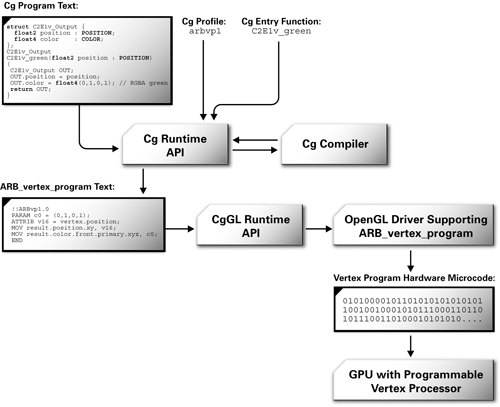
\includegraphics[width=1\linewidth]{fig2_2.jpg}
    \caption{Compiling and Loading a Cg Program into the GPU}
    \label{fig:2-2}
\end{figure}

Once loaded with a vertex program, the programmable vertex processor in your GPU runs that program every time the application feeds a vertex to the GPU. When it renders a complex model with thousands of vertices, your current vertex program processes every vertex in the model. The vertex program runs once for each vertex.

A single current vertex program is loaded in the programmable vertex processor for execution at any one time. However, your application may change the current vertex program, as needed.

This same concept of a single current program applies to the programmable fragment processor in your GPU too. You compile your Cg fragment program and use the Cg runtime, along with your 3D programming interface, to download your program and bind it as the current fragment program for processing fragments generated by the rasterizer. After your fragment program is bound, 3D primitives are rasterized into fragments and your current fragment program processes each generated fragment. The fragment program runs once for each fragment.

Typically, 3D applications co-program the programmable vertex and fragment processors in the GPU to achieve a particular rendering effect. This approach is very efficient because of the parallel and highly pipelined nature of the programmable vertex and fragment processors in GPUs.

\section{A Simple Fragment Program}

So far, our example involves only a vertex program, \textbf{C2E1v_green}. This section presents a simple fragment program that you can use with our vertex program.

Example 2-2 shows the complete Cg source code for our first fragment program.

\FloatBarrier
\begin{lstlisting}[caption=Example 2-2. The \textbf{C2E2f_passthrough} Fragment Program]
struct C2E2f_Output {
  float4 color : COLOR;
};

C2E2f_Output C2E2f_passthrough(float4 color : COLOR)
{
  C2E2f_Output OUT;
  OUT.color = color;
  return OUT;
}
\end{lstlisting}
\FloatBarrier

This program is even simpler than the example for the \textbf{C2E1v_green} vertex program. In fact, it does almost nothing. The program outputs the unchanged interpolated color assigned for every fragment generated by the rasterizer. The GPU's raster operation hardware uses this color to update the frame buffer if the fragment survives the various raster operations, such as scissoring and depth testing.

Here is the output structure returned by \textbf{C2E2f_passthrough}:

\FloatBarrier
\begin{lstlisting}
struct C2E2f_Output {
  float4 color : COLOR;
};
\end{lstlisting}
\FloatBarrier

Fragment programs have a simpler output structure than vertex programs. A vertex program must output a position and may return one or more colors, texture coordinate sets, and other per-vertex outputs. A fragment program, however, must reduce everything to a single color that will update the frame buffer. (In some advanced profiles, fragment programs can write additional data such as a depth value as well.) The \textbf{COLOR} semantic assigned to the \textbf{color} member in a fragment program indicates that the member is the color to be used to update the frame buffer.

The entry function declaration for \textbf{C2E2f_passthrough} is this:

\FloatBarrier
\begin{lstlisting}
C2E2f_Output C2E2f_passthrough(float4 color : COLOR)
\end{lstlisting}
\FloatBarrier

The function returns the \textbf{C2E2f_Output} output structure with one color. The function receives a single four-component vector, named "color," bound to the \textbf{COLOR} input semantic. The \textbf{COLOR} input semantic for a fragment program is the color of the fragment interpolated by the rasterizer, based on the primitive's assigned vertex colors.

The body of \textbf{C2E2f_passthrough} is this:

\FloatBarrier
\begin{lstlisting}
{
  C2E2f_Output OUT;
  OUT.color = color;
  return OUT;
}
\end{lstlisting}
\FloatBarrier

After declaring an \textbf{OUT} variable with the \textbf{C2E2f_Output} output structure type, the program assigns the fragment's interpolated color (the single input parameter) to the final fragment color in the output structure. Finally, the program returns the \textbf{OUT} structure.

\subsection{Fragment Program Profiles}

Just as you needed a profile to compile the \textbf{C2E1v_green} example, you also need a profile to compile the \textbf{C2E2f_passthrough} example. However, the profiles for compiling the \textbf{C2E1v_green} example were for vertex programs. To compile \textbf{C2E2f_passthrough} , you must choose an appropriate fragment profile.

Table \ref{table:2-2} lists various profiles for compiling fragment programs.

\begin{table}
\centering
\begin{tabular}{ |c|c|c|c|c|c|c|c| } 
 \hline
Profile Name & Programming Interface & Description \\
ps_1_1 ps_1_2 ps_1_3 & DirectX 8 & Basic multivendor fragment programmability \\
fp20 & OpenGL & Basic NVIDIA fragment programmability (corresponding to NV_texture_shader and NV_register_combiners functionality) \\
arbfp1 & OpenGL & Advanced multivendor fragment programmability (corresponding to ARB_fragment_program functionality) \\
ps_2_0 ps_2_x & DirectX 9 & Advanced multivendor fragment programmability \\
fp30 & OpenGL & Advanced NVIDIA fragment programmability (corresponding to NV_fragment_program functionality) \\
 \hline
\end{tabular}
\caption{Cg Fragment Profiles}
\label{table:2-2}
\end{table}

Like the earlier vertex program example, this first fragment program example is so simple that you can compile the \textbf{C2E2f_passthrough} example with any of the profiles in Table \ref{table:2-2}.

Cg has a command-line compiler known as \textbf{cgc}, which is short for "Cg compiler." Dynamic compilation at runtime can be very powerful and is highly recommended. However, when you are writing Cg programs, you often want to verify that they compile correctly without having to run your 3D application. To detect Cg compiler errors while writing programs, try running \textbf{cgc}. It will "test compile" the Cg program files used by your application as part of your regular application build process. Using \textbf{cgc} in an integrated development environment (IDE) such as Microsoft's Visual C++ can make it quick and easy to find compilation errors. A good IDE will even help you quickly locate the appropriate line of code, based on line numbers in the error message, just as you would with C or C++ programs. Figure \ref{fig:2-3} shows an example of debugging compiler errors in Microsoft Visual Studio.

\begin{figure}
    \centering
    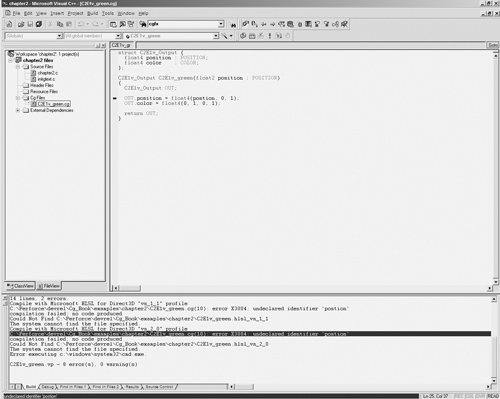
\includegraphics[width=1\linewidth]{fig2_3.jpg}
    \caption{Locating Error Lines in an Integrated Development Environment}
    \label{fig:2-3}
\end{figure}

\subsection*{Coding Tip}

Cg developers often write a single Cg program that works for both OpenGL and Direct3D, even if they predominantly use one programming interface or the other. However, profile-dependent differences can exist between what is valid in the corresponding profiles for these 3D programming interfaces. So make it your practice to compile your Cg programs twice with \textbf{cgc}: once for the appropriate OpenGL profile, and again for the appropriate Direct3D profile.
\hrule

\section{Rendering with Your Vertex and Fragment Program Examples}

Now it's time to see your two simple Cg programs in action. Don't expect too much, because these are both very simple programs. However, you can still learn a lot by examining how the programs work together—and with the rest of the graphics pipeline—to draw a green triangle.

Look at the 2D triangle in Figure \ref{fig:2-4}. This is the geometry that your vertex and fragment program will operate on in this example.

\begin{figure}
    \centering
    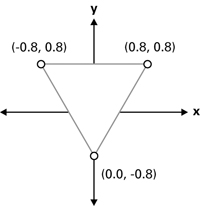
\includegraphics[width=0.5\linewidth]{fig2_4.jpg}
    \caption{A 2D Triangle for Rendering}
    \label{fig:2-4}
\end{figure}

\subsection{Rendering a Triangle with OpenGL}

In OpenGL, you can render this 2D triangle with the following commands:

\FloatBarrier
\begin{lstlisting}
glBegin(GL_TRIANGLES);
  glVertex2f(-0.8, 0.8);
  glVertex2f(0.8, 0.8);
  glVertex2f(0.0, -0.8);
glEnd();
\end{lstlisting}
\FloatBarrier

\subsection{Rendering a Triangle with Direct3D}

In Direct3D, you can render the same triangle with the following code:

\FloatBarrier
\begin{lstlisting}
D3DXVECTOR4 vertices[3] =
{
    D3DXVECTOR4(-0.8f,  0.8f, 0.f, 1.f),
    D3DXVECTOR4( 0.8f,  0.8f, 0.f, 1.f),
    D3DXVECTOR4( 0.0f, -0.8f, 0.f, 1.f),
};

m_pD3DDevice->DrawPrimitiveUP(D3DPT_TRIANGLELIST, 1,
  vertices, sizeof(D3DXVECTOR4));
\end{lstlisting}
\FloatBarrier

There are other, more efficient ways to transfer vertices to the GPU in OpenGL or Direct3D. When you use Cg programs to process vertices, it doesn't matter how the application sends the vertices to the GPU.

\subsection{Getting the Same Results}

Figure \ref{fig:2-5} shows the result of rendering this triangle with the \textbf{C2E1v_green} vertex program and \textbf{C2E2f_passthrough} fragment program configured. The result is the same, whether rendered with OpenGL or Direct3D. Admittedly, it's not very exciting, but the triangle is solid green.

\begin{figure}
    \centering
    
\includegraphics[width=0.25\linewidth]{fig_0006.jpg}
    \caption{Rendering a Triangle with \textbf{C2E1v_green} and \textbf{C2E2f_passthrough}}
    \label{fig:2-5}
\end{figure}

The vertex program passes the specified 2D position of each vertex to the rasterizer. The rasterizer expects positions to be specified as coordinates in clip space. Clip space defines what is visible from the current viewpoint. If the vertex program supplies 2D coordinates, as is the case in Figure \ref{fig:2-5}, the portion of the primitive that is rasterized is the portion of the primitive where x and y are between -1 and +1. The entire triangle is within the clipping region, so the complete triangle is rasterized.

Figure \ref{fig:2-6} shows the region of rasterization for 2D clip space.

\begin{figure}
    \centering
    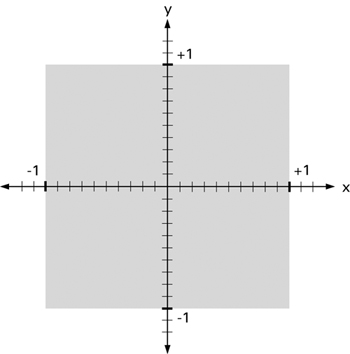
\includegraphics[width=0.5\linewidth]{fig2_6.jpg}
    \caption{A 2D View of Clip Space}
    \label{fig:2-6}
\end{figure}

Primitives are rendered into the frame buffer if they fall within the gray region (the region of clip space where x and y are between -1 and +1). You'll learn more about clip space in Chapter 4.

Figure \ref{fig:2-7} shows what happens when you use the \textbf{C2E1v_green} vertex program and \textbf{C2E2f_passthrough} fragment program with 2D geometry that is not entirely within the visible region of 2D clip space. When the stars include vertices that have x or y coordinates outside the -1 to +1 region, the rasterizer clips some of the green stars by the edge of the visible region. If no part of a primitive is within the viewable region of clip space, the rasterizer eliminates the primitive.

\begin{figure}
    \centering
    
\includegraphics[width=0.25\linewidth]{fig_0008.jpg}
    \caption{Primitives Rendered with and Require 2D Clipping}
    \label{fig:2-7}
\end{figure}

The GPU then transforms clip space automatically (by a simple scale and bias) into window space coordinates for the rasterizer. Effectively, the GPU stretches clip-space coordinates as necessary, prior to rasterization, to fit the rendering viewport and window position.

Chapter 4 generalizes this 2D notion of clip space to 3D, and includes perspective views. But in this chapter and Chapter 3, the examples use 2D rendering to keep things simple.

\section{Exercises}

\FloatBarrier
\begin{enumerate}
\item \textbf{Answer this:} What GPU profiles does your Cg compiler support? Consult your compiler's documentation or try running \textbf{cgc –help} at the command line. Which profiles are vertex profiles and which are fragment profiles?
\item \textbf{Try this yourself:} Modify the \textbf{C2E1v_green} vertex program to color the vertices red instead of green.
\item \textbf{Try this yourself:} Change the one triangle vertex position by extending the vertex coordinates outside the [-1, +1] range. Run the example. Is the triangle clipped as you would expect?
\end{enumerate}
\FloatBarrier

\section{Further Reading}

Check out the documentation, such as the \textit{Cg Toolkit User's Manual: A Developer's Guide to Programmable Graphics}, that accompanies the Cg Toolkit software distribution.

Also, visit the Web site \textbf{www.cgshaders.org} for current Cg information. This site has articles, forums where you can ask questions, and freely available sample shader code.

\end{document}